\Chapter{Elméleti háttér}

Szakdolgozatom célja létrehozni egy olyan kliens-szerver weboldalt, amely bárki számára könnyen használható és látványos kimutatásokat tud ezáltal készíteni. Már a tervezési fázisban elhatároztam, hogy a weboldal felépítése hasonlítani fog a kutatásom során megismert tőszdei témájú weboldalakhoz, mind felépítésében, mind megvalósításában, hogy a felhasználó azt érezze egy\textit{ élő és lélegző weboldal}on böngészik. Ehhez viszont előtte szeretném ismertetni a szakdolgozatomhoz szükséges tudáshátteret.

\Section{Grafikonok története és típusai}

Egy látványos grafikonnal könnyebb bemutatni egy elemzést, vagy történetet, mint szóban elmesélni. Ugyan ma alapkellékként értelmezzük a vonaldiagrammokat és kördiagrammokat, viszont egykor forradalmi újításnak számítottak. Volt rá példa, hogy használatuk szó szerint életbevágónak bizonyult, amikor egy angol orvosnő, diagrammok segítségével győzte meg a férfiak által vezetett orvosközösséget, hogy jobban oda kell figyelni a kórházi higiéniára. A kifogástalan és figyelem felkeltő grafikonjának hála, katonák tömegei élték túl a krími háborút.  \cite{portfolio}

	A grafikon a diagram egyik fajtája, amely két adat kapcsolatát egy derékszögű koordináta-rendszerben ábrázolja. A két tengely jelképezi a két adatot, és a grafikon jelzi, hogy az egyik adatnak az egyes értékeihez a másik mely értékei tartoznak. Általában két mennyiség közötti lineáris kapcsolatot, vagy egy mennyiség időbeli változásának bemutatására használják. Matematikai szemszögből a grafikon egy függvényt ábrázol. \cite{wikiMatek}

\begin{figure}[h]
\centering
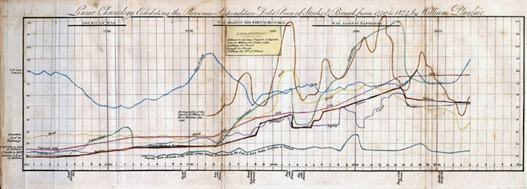
\includegraphics[scale=1]{images/historyOfGraphs}
\caption{Az egyik első statisztikai gráf (forrás: \cite{oldGraph})}
\end{figure}

\SubSection{Grafikon típusok \cite{graphTypes}} 

\subsubsection{Vonaldiagram}

A vonaldiagram olyan grafikon, amely vonalakat használ az egyes adatpontok összekapcsolására. A vonaldiagram kvantitatív értékeket jelenít meg egy meghatározott időintervallumban. A pénzügyekben a vonaldiagrammokat általában egy eszköz vagy értékpapír történelmi árfolyamműveletének ábrázolására használják. 

	Működését tekintve egy vonal köti össze az egyes adatpontokat, amelyek jellemzően mennyiségi értékeket jelenítenek meg. Befektetések terén a technikai elemzés területén a vonalgrafikonok meglehetősen informatívak, lehetővé téve a felhasználó számára a trendek megjelenítését. Míg a vonaldiagrammokat sok különböző mezőben használják különböző célokra, leggyakoribb funkciójuk az értékek időbeli változásainak grafikus ábrázolása.

\begin{figure}[h]
\centering
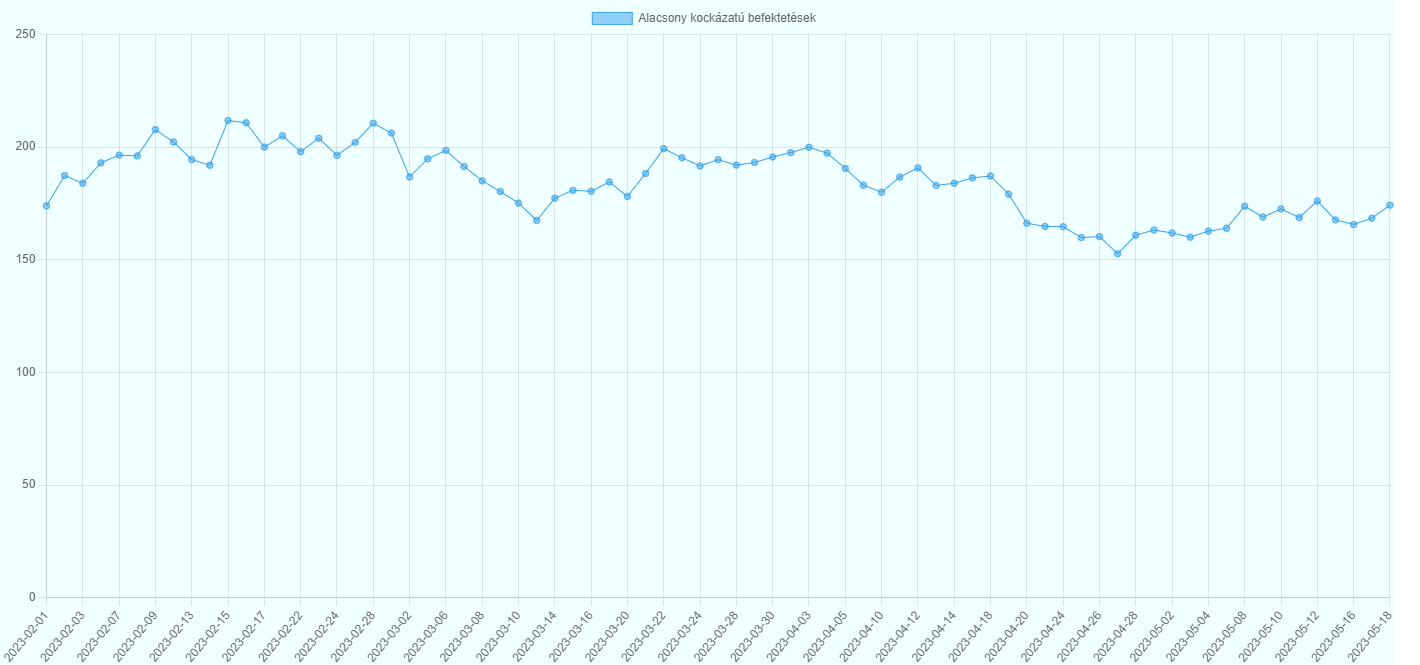
\includegraphics[scale=0.3]{images/lineChartExample}
\caption{Általam készített grafikonrajzoló oldalán megjelenített vonaldiagram}
\end{figure}

\subsubsection{Oszlopdiagram}

Az oszlopdiagram az információ grafikus ábrázolására szolgál. Különböző magasságú sávokat használ az értékek kimutatására. 

	Működését tekintve oszlopdiagrammokat létre lehet hozni függőleges sávokkal, vízszintes sávokkal, csoportos sávokkal (több sáv, amelyek egy kategória értékeit hasonlítják össze) vagy halmozott sávokkal (több típusú információt tartalmazó oszlopok). A sávok egy adott adatkategória értékét jelenítik meg az hatázorra meg annak méretét. Az oszlopdiagramokat általában az üzleti és pénzügyi elemzésekben használják a gyakran bonyolult adatok megjelenítésére, mivel gyorsan és hatékonyan tudnak információt közvetíteni.

\clearpage

\begin{figure}[h]
\centering
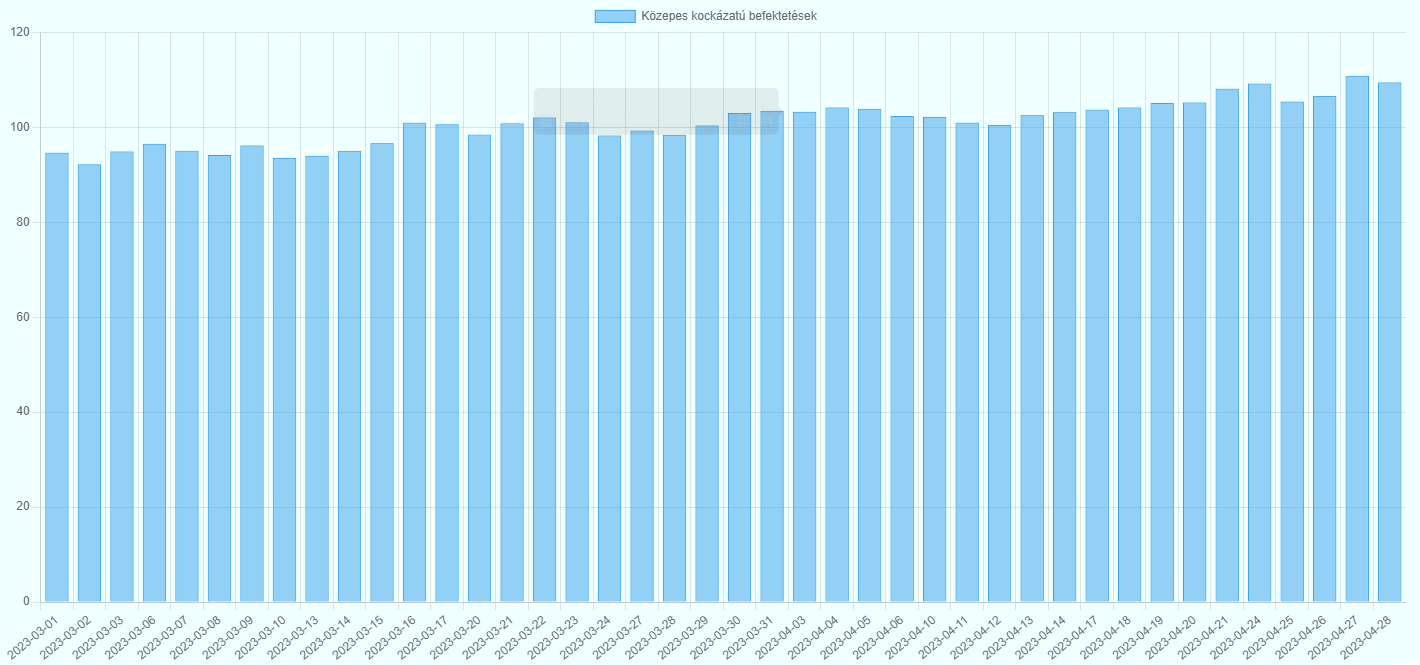
\includegraphics[scale=0.3]{images/barChartExample}
\caption{Általam készített grafikonrajzoló oldalán megjelenített oszlopdiagram}
\end{figure}

\subsubsection{Kördiagram}

A kördiagram egy névleges adathalmaz összegzésének vagy egy adott változó különböző értékeinek megjelenítésének módja (pl. százalékos eloszlás). A kördiagrammok használata meglehetősen népszerű, mivel a kör vizuális koncepciót ad az egészről. Egyik alfaja a poláris diagram.

	Működését tekintve az ilyen típusú diagram egy szegmenssorozatra osztott kör. Minden szegmens egy adott kategóriát képvisel. Az egyes szegmensek területe a körnek ugyanolyan arányban van, mint a kategória a teljes adatkészletben.

\begin{figure}[h]
\centering
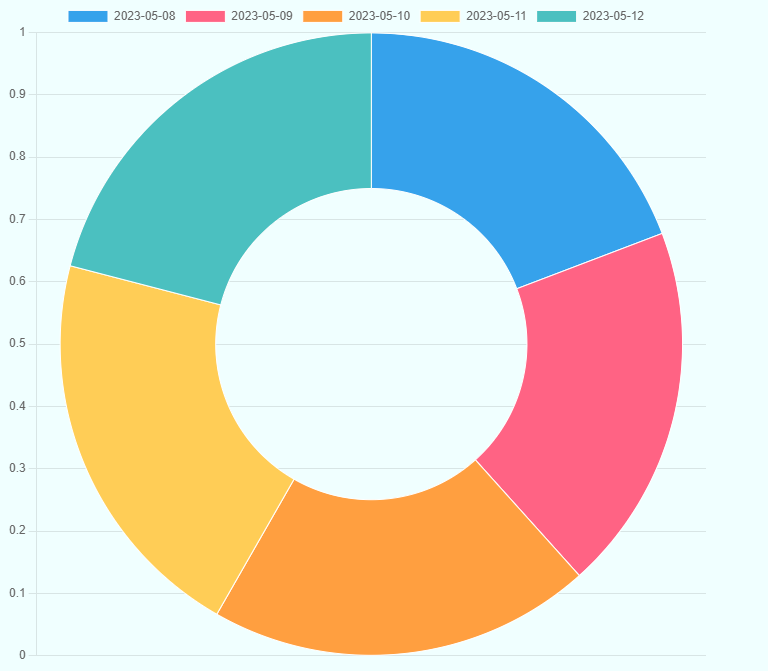
\includegraphics[scale=0.4]{images/pieChartExample}
\caption{Általam készített grafikonrajzoló oldalán megjelenített kördiagram}
\end{figure}

\subsubsection{Radardiagram}

A radardiagram segít szemléltetni a különböző jellemzőkkel rendelkező adatcsoportok összehasonlítását. Segítségével könnyen össze lehet mérni másfajta paraméterekkel rendelkező elemeket. 

	Működését tekintve az adatokat ugyanarra a központi pontra helyezi, és átlátszó árnyalatokkal és mintákkal mutatja be a kontrasztot az olvasó számára. Egy adott pont értékének nagyságát az jelzi, minél távolabbra nyúlik az origótól a pókháló szerű diagrammon.

\begin{figure}[h]
\centering
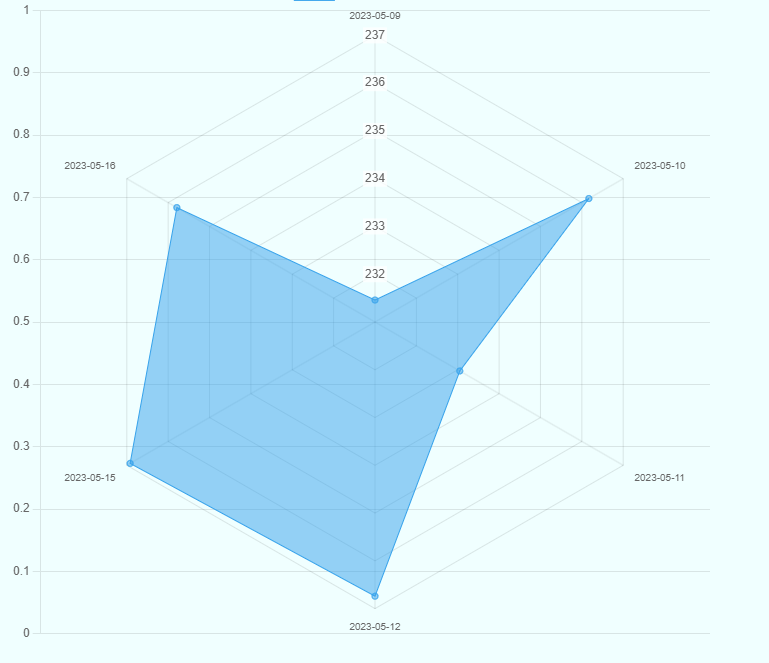
\includegraphics[scale=0.4]{images/radarChartExample}
\caption{Általam készített grafikonrajzoló oldalán megjelenített radardiagram}
\end{figure}

\Section{Tőzsde}

A tőzsde talán a modernt világ egyik legjobban félreértelmezett kifejezése.A hétköznapi ember lelki szemei előtt számok végtelen sokasága lebeg, amikor meghallja és csak legyint rá, hogy ez számára túl komplikált, ahhoz, hogy átlássa és megértse. Nos, ez az állítás részben igaz is, hiszen lehet nagyon bonyolult a tőzsde, viszont lehet nagyon egyszerű is.

	A tőzsde egy olyan nyilvános, központosított és szervezett piac, ahol meghatározott árukat, meghatározott időben, azon belül meghatározott személyek adhatnak, vagy vehetnek szigorú eljárási szabályok szerint.  Ez mit is jelent a gyakorlatban? A tőzsde is egy olyan piac, mint amilyet akármelyik városban, vagy faluban találhatunk. A különbség az, hogy vásárlás során maga az áru nem materiális formában jelenik meg, illetve nem csak az adott környezettel, hanem az egész világgal lehetőségünk van kereskedni. Viszont, hogy mibe érdemes fektetni az bonyolultabb, mint elsőre képzelnénk.  \cite{wikiStock}
	
A tőzsdék fajtái lehetnek: 

\begin{itemize}
\item Árutőzsde
\item Értéktőzsde, ezen belül: 
	\begin{itemize}
	     \item Devizatőke
	     \item Értékpapírtőzsde 
	     \item Hírpiac
	\end{itemize}
\end{itemize}

\SubSection{Részvény}

A részvény tulajdonjogot és egyéb gazdasági jogokat megtestesítő értékpapír, nincsen lejárati ideje. Ezeket az értékpapírokat a részvénytársaságok a részvény birtokosainak, annak részesedése arányában osztják szét jövedelem és szavazati jogok arányos formájában.

	A részvények nagyobbrészt névre szóló értékpapírok, amelyeket leginkább elektronikus úton, dematerizált formában állítanak elő, hogy kereskedelmi forgalomba hozhatóak legyenek. A fizikai értékpapírok tárolása leginkább bankokban, vagy takarékszövetkezetekben történik. A részvényekkel tőzsdén kívüli piacokon is kereskednek, amelyekre általában lazább szabályok vonatkoznak, mint a központosított piacokon. 

	A részvénytulajdonlás jövedelem növelése érdekében történik. Egy vállalat termelő, vagy szolgáltató tevékenységének célja a profitszerzés, hogy ezt elérhetővé tegye részvénytársasággá kell vállalnia. A vállalkozásban lévő részesedést az alapító tagok között szokás meghatározni, hogy mely tag mekkora összeggel járult hozzá az adott vállalkozás elindításához. Abban az esetben, ha csak az alapítók rendelkeznek részesedéssel, akkor zárt részvénytársaságról beszélünk. Amennyiben az alapítók úgy határoznak, hogy a céget a nyilvánosság elé tárják, akkor zártkörű helyett a cég elkezd részvényeket kibocsájtani. Ezen részvények összessége arányos azzal a tulajdonjoggal, amiről az alapítók lemondtak.

	Többfajta részvénytípusok elérhetőek, a teljesség igénye nélkül felsorolok párat, például: befektetési életbiztosítások, \textbf{befektetési alapok}, nyugdíj célú megtakarítások.  \cite{wikiShare}

\Section{Befektetési alapok}

Azon személyek, akik pénzüket beszerették volna fektetni valamilyen szolgáltatásba, már nagy eséllyel hallottak a befektetési alapokról. Ezen termékek kedvezőek és meggyőzőek lehetnek bárki számára. A tőzsde egyik „alapszabálya”, hogy befektetéskor nem ajánlott egyetlen terméket vásárolni. A diverzifikáció ugyanis nagyon fontos, hiszen nem csak ezzel csökkenthetjük a kockázatot, hanem sokkal több tapasztalatot is tudunk gyűjteni és minél több csapot nyit meg a befektető annál nagyobb eséllyel lesz sikeres. \cite{OTPInvest}

	A befektetési alap olyan vagyontömeg, amely állhat értékpapírból, ingatlanokból, bankbetétekből és részvényekből. Befektetési alapot csakis befektetési alapkezelő hozhat létre és kezelhet. Egy befektetési alapkezelő több befektetési alapot is kezelhet. A befektetési alapok futamideje változó, beszélhetünk akár pár hónapos futamidőről, de akár évtizedekig tartó időintervallumról is. A rövid futamidejű alapokat likvidálási alapoknak hívjuk és mindig nyitott végű alapok. Mit jelent az a kifejezés, hogy \emph{nyitott végű alap}ok? 

	A befektetésí alapokat két fajta típus alapján különböztetjük meg, ezen típusok jelzik, hogyan lehet csatlakozni egy alaphoz.
\begin{itemize}
\item \textbf{Nyíltvégű alapok}: bármelyik forgalmazási napon lehetőségünk nyílik csatlakozni, illetve vissza is válthatjuk belőle a megtakarításainkat. Ezek az alapok általában határozatlan futamidőre jönnek létre és mi dönthetjük el, meddig tartjuk bent a megtakarított pénzünket. Mindig érdemes figyelni a javasolt befektetési időtávokat, hogy a befektetésünk jó eséllyel az elvárt teljesítményt tudja nekünk szolgáltatni.
\item \textbf{Zártvégű alapok}: a zártvégű alapokhoz csak az alap indulása előtti jegyzési időszakban van lehetőségünk csatlakozni. Ezen alapok általában határozott futamidőre jönnek létre, tehát az alap lejárattal rendelkeznek, ezen időszakig a megtakarításainkat az alapban kell tartanunk. Természetesen, ha a futamidő alatt mégis szükségünk lenne a befektetett összegre, a zártvégű alapokat tőzsdei megbízás útján értékesíteni tudjuk, ilyenkor a pillanatnyi kereslet fogja meghatározni a befektetésünk ellenértékét, nem pedig annak az értéke. Ezért, fontos jól megfontolni, ha zártvégű alapot választunk, célszerű és javaslott a befektetésünket a lejáratig megtartani.  

Az alapokat az alapján is csoportosíthatjuk, hogy azok milyen típusú eszközbe fektetik a befektetők megtakarításait.  

\end{itemize}
\begin{itemize}
\item \textbf{Pénzpiaci befektetési alap}: pénzpiaci alapok, állampapírok és különböző banki betétek.
\item \textbf{Kötvényalapok}: különböző kötvények vásárolhatók.
\item \textbf{Részvényalapok}: vállalatok által kibocsátott részvények.
\item \textbf{Vegyes alapok}: többféle portfólióban csoportosított részvények és  kötvények.
\item \textbf{Ingatlan befektetési alap}: már megépült vagy építésben levő ingatlanokba való befektetés.
\item \textbf{Speciális befektetési alapok}: abszolút hozamú, tőkevédett és származtatott alapok. 
\end{itemize}

	Mivel ilyen sokrétű lehet egy befektetési alap, így felmerülhet a vásárlóban, hogy miért érdemes befektetési alapba fektetnie a pénzét? Erre a kérdésre az egyik legjobb érv a kockázatmegosztás. Ugyanis már egyetlen befektetési alap megvásárlásával is több egyedi értkékpapírból álló, szakszerűen összeállított portfólióhoz juthatunk hozzá, amit egyéni befektetőként rengeteg idő és erőfeszítés árán révén érhetnénk el. Amennyiben befektetési alapot választunk megtakarításaink elhelyezésére nincsen más dolgunk, mint vásárolni az alap befektetési jegyeiből. Ezzel az egyszerű tranzakcióval gyakorlatilag megbízunk egy szakértői gárdát, akik az összes a befektetésünkkel kapcsolatos terhet levesznek a vállunkról, és különféle értékpapírokba helyezik el megtakarításaikat.

\begin{figure}[h]
\centering
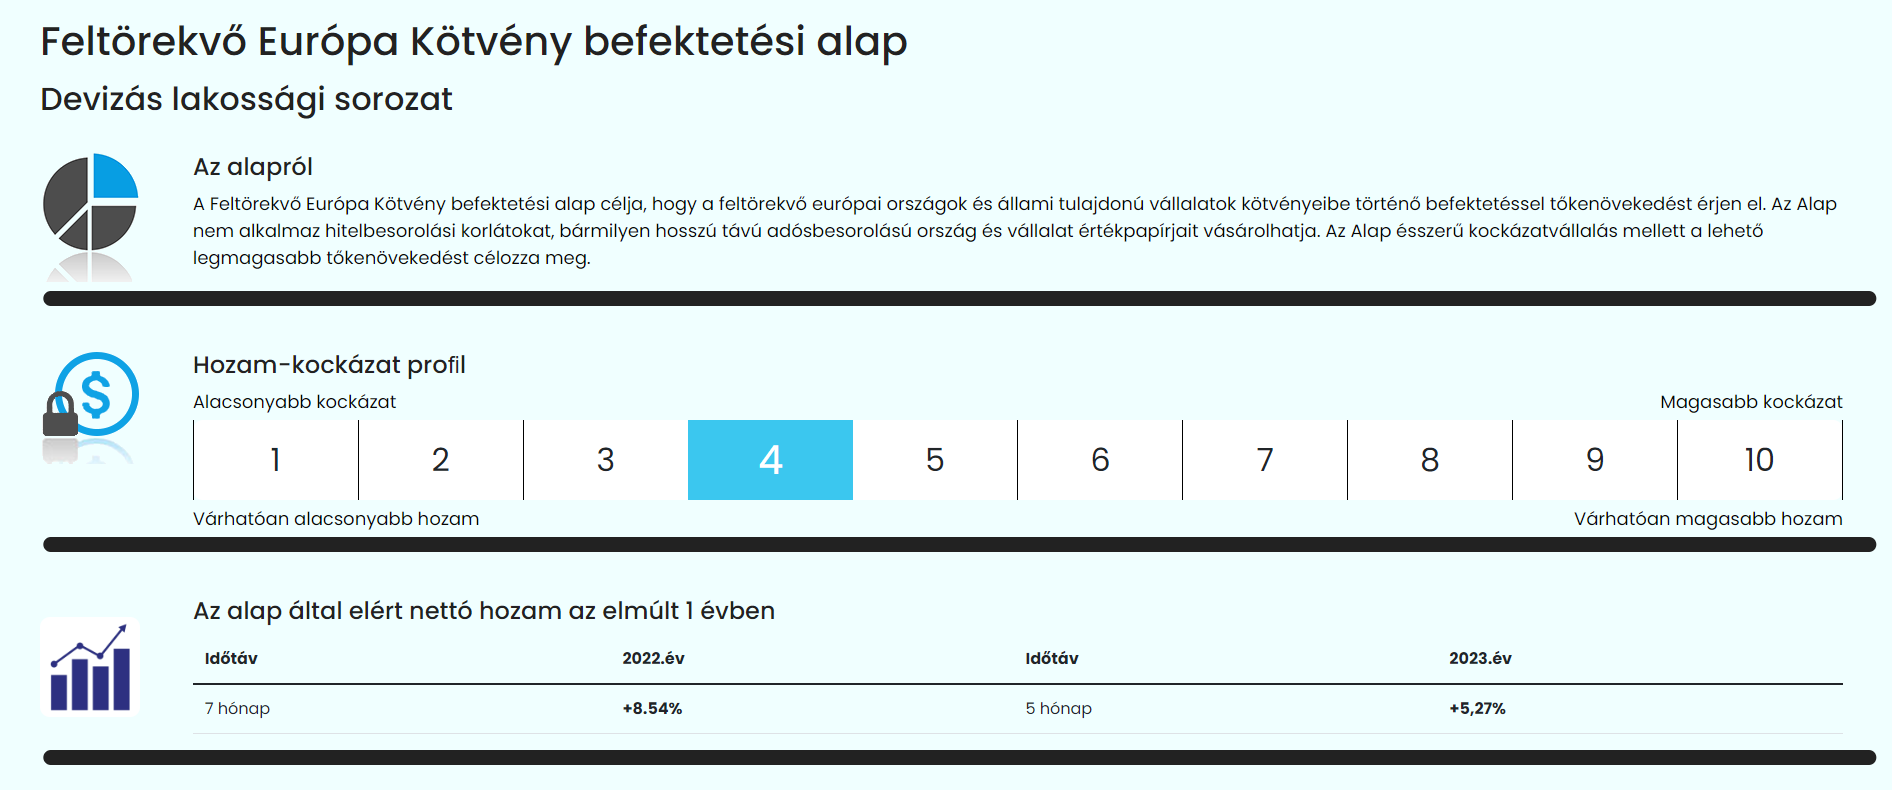
\includegraphics[scale=0.3]{images/europeInvestExample}
\caption{Általam készített weboldal egyik befektetési alapja}
\end{figure}

\SubSection{Tőzsdei árfolyam }

Tőzsdei árfolyamoknak nevezett árfolyamokat a globális pénzügyi piacon határozzák meg, ahol a bankok és más pénzügyi intézmények éjjel-nappal kereskednek valutákkal ezen tényezők alapján. Az árfolyamot általában az általa képviselt nemzeti valuta betűszóval jegyzik, mint például a leggyakrabban használt valuta az \emph{USD}, ami az amerikai dollárt jelenti. Mérésének számos módja van, a  leggyakoribb módszer a kétoldalú árfolyam mérése. A bilaterális árfolyam az egyik valuta másikhoz viszonyított értékére vonatkozik. A tőzsdén található árfolyamoknak több típusát különböztetjük meg, ezek az alábbiak lehetnek: 
\begin{itemize}
\item Nyitó árfolyam
\item Napi maximum érték
\item Napi minimum érték
\item Napi záró érték
\item Napi átlag érték \cite{exchangeRate}
\end{itemize}

